%---------------------导言区---------------------------%
\documentclass[12pt,a4paper,UTF8]{ctexart}
	%10pt：正文字体为12pt，缺省为10pt；各层级字体大小会根据正文字体自动调整
	%a4paper：纸张大小a4；
	%UTF8：中文要求
\usepackage{geometry}%用于设置上下左右页边距
	\geometry{left=2.5cm,right=2.5cm,top=3.2cm,bottom=2.8cm}
\usepackage{xeCJK}
\usepackage{amsmath}
\usepackage{paralist}
\usepackage{enumerate}
\usepackage{booktabs}
\usepackage{multirow}
\usepackage{graphicx}
\usepackage{subfig}
\usepackage{setspace}
\usepackage{listings}
\usepackage{lastpage}
\usepackage{hyperref}
\usepackage{pdfpages}

%xeCJK：中文字体（如楷体，作者和机构需要用到）的设置
	%amsmath：数学公式
	%paralist，enumerate：自定义项目符号
	%booktabs：三线图，论文常用的表格风格
	%multirow：复杂表格
	%graphicx，float: 插入图片
	%subfig：并排排版图片、竖向排版图片
	%setspace：设置行间距等功能
	\setlength{\parindent}{2em}%正文首行缩进两个汉字
	%listings:用于排版各种代码；比如matlab的代码
	\lstset{language=Matlab}%matlab代码
	%lastpage:获取总页数;
	%hyperref:超链接,和lastpage搭配.
\usepackage{fancyhdr}
	%fancyhdr：一个很强大的宏包，用于自定义设计页面风格并命名以供调用。
	\pagestyle{fancy}
	\rhead{电光调制及光通讯模拟实验}
	\lhead{近代物理实验~~~实验报告}
	\cfoot{Page \thepage/\pageref{LastPage}}  %当前页\总页数
	\rfoot{\today}
		%分别是右页眉、左页眉、中页脚、右页脚
	\renewcommand{\headrulewidth}{0.4pt}
	\renewcommand{\theenumi}{(\arabic{enumi})}

%%%%%%%%%%%%%%%%%%%%%%%%%%%%%%%%%%%%%%%%%%%%%%%%%%%%%%%%%%
%%%%%%%%%%%%%%%%%%%%%%%%%正文开始%%%%%%%%%%%%%%%%%%%%%%%%%%
%%%%%%%%%%%%%%%%%%%%%%%%%%%%%%%%%%%%%%%%%%%%%%%%%%%%%%%%%%

\begin{document}

%%begin-------------------标题与信息-----------------------%%

%%标题
\begin{center}
\LARGE\textbf{电光调制及光通讯模拟实验}
\end{center}

%%信息
\begin{doublespacing}
	%doublespacing：手动两倍行距
	\begin{tabular}{lr}
	 & \\
	 {实验人姓名：徐殊行~23343071} & {合作者姓名：王志超~23343062}\\
	 {实验时间：2025年3月7日, 3月14日} & {室温：28$^{\circ}$C~相对湿度：59\%}
	
	\end{tabular}
\end{doublespacing}

%%-------------------中英文摘要-----------------------%%
\begin{abstract}
	本实验研究了电光调制及其在通讯领域的应用。通过实验，我们观察了铌酸锂晶体的电光效应，并测量了其半波电压、电光系数、透过率等关键参数。
	实验采用了极值法测量半波电压，并通过透过率曲线分析调制器的线性工作区。
	此外，我们探讨了倍频失真现象，并利用会聚偏振光干涉实验分析了电场对晶体光学性质的影响。
	本实验加深了对电光效应及其在光学调制中的应用的理解，为光通讯技术提供了重要的实验基础。

	\noindent \textbf{关键词：电光调制、电光效应、半波电压、透过率} 
		
\end{abstract}
	
\renewcommand{\abstractname}{Abstract}

\begin{abstract}
	This experiment studies electro-optic modulation and its applications in communication. 
	Through the experiment, we observed the electro-optic effect of lithium niobate crystals and measured key parameters 
	such as half-wave voltage, electro-optic coefficient, and transmittance. 
	The half-wave voltage was measured using the extremum method, and the linear working region of the modulator was analyzed through the transmittance curve. 
	Additionally, we explored the phenomenon of frequency doubling distortion and analyzed the effect of the electric field on the optical properties of the crystal 
	using converging polarized light interference experiments. 
	This experiment deepens the understanding of the electro-optic effect and its applications in optical modulation, 
	providing an important experimental foundation for optical communication technology.

	\noindent \textbf{Keywords:~~Electro-optic modulation~~~Electro-optic effect~~~Half-wave voltage~~~Transmittance}
\end{abstract}


%%-------------------正文部分-----------------------%%

\subsection*{【实验目的】}

\begin{enumerate}[(1)]
	\item 学习晶体的电光调制的实验原理并掌握实验方法
	\item 学习用调制器的特性曲线测量半波电压的方法
	\item 测量电光调制器的消光比，透过率等参数
\end{enumerate}


\subsection*{【实验原理】}

\subsubsection*{1.各向异性晶体的折射率}
	根据光的电磁理论，光是一种电磁波，在介质中传播的速度为

	\begin{equation}
	    c = \frac{c_0}{n} = \frac{1}{\sqrt{\mu \varepsilon}},
	\end{equation}

	其中，$n^2 = \varepsilon / \varepsilon_0$，$\varepsilon$ 为介电系数，是对称的二阶张量，即 $\varepsilon_{ij} = \varepsilon_{ji}$。因此在各向异性的介质中，电位移矢量与电场的关系可以表述为：
	
	\begin{equation}
	    \begin{pmatrix} D_x \\ D_y \\ D_z \end{pmatrix} = \varepsilon_0 \begin{pmatrix} \varepsilon_{xx} & \varepsilon_{xy} & \varepsilon_{xz} \\ \varepsilon_{yx} & \varepsilon_{yy} & \varepsilon_{yz} \\ \varepsilon_{zx} & \varepsilon_{zy} & \varepsilon_{zz} \end{pmatrix} \begin{pmatrix} E_x \\ E_y \\ E_z \end{pmatrix}.
	\end{equation}

	对于任意一种晶体，我们总可以找到三个相互正交的特殊方向 $(x, y, z)$，使介电张量对角化，即：

	\begin{equation}
    	\begin{pmatrix} D_x \\ D_y \\ D_z \end{pmatrix} = \varepsilon_0 \begin{pmatrix} \varepsilon_x & 0 & 0 \\ 0 & \varepsilon_y & 0 \\ 0 & 0 & \varepsilon_z \end{pmatrix} \begin{pmatrix} E_x \\ E_y \\ E_z \end{pmatrix}.
	\end{equation}

	这三个特殊的方向称为晶体的主轴方向，在这三个主轴方向上有：

	\begin{equation}
	    D_i = \varepsilon_0 \varepsilon_i E_i, \quad (i = x, y, z),
	\end{equation}
	
	对应的三个主折射率为：
	
	\begin{equation}
	    n_i = \sqrt{\varepsilon_i}, \quad (i = x, y, z).
	\end{equation}

	在各项同性的介质中，\(\epsilon_{x} = \epsilon_{y} = \epsilon_{z} = \epsilon\)，电位移矢量和电场矢量成简单的线性关系，光在这类介质中以同一速度传播。
	在各向异性的介质中，各方向的折射率不同，所以各偏振态的光传播速度也不同，呈现双折射现象，通常用折射率椭球来描述折射率与光的传播方向、振动方向的关系。

\subsubsection*{2.电光效应}
	电光效应主要分为两类：线性电光效应（Pockels 效应）和二次电光效应（Kerr 效应）。
	Pockels 效应是由外加电场的一次项引起的折射率变化，通常发生在无中心对称的晶体中，由 Pockels 于 1893 年发现。
	Kerr 效应则是由电场的二次项引起的变化，一般存在于各类介质中，由 Kerr 于 1875 年发现。
	通常，在无对称中心的晶体中，线性电光效应要远强于二次电光效应，因此在电光调制应用中，通常讨论线性电光效应。
	
	当晶体加上电场后，折射率椭球的形状、大小、方位都会发生变化，椭球方程变为：
	\begin{equation}
	    \frac{x^2}{n_x^2} + \frac{y^2}{n_y^2} + \frac{z^2}{n_z^2} + \frac{2yz}{n_{yz}^2} + \frac{2xz}{n_{xz}^2} + \frac{2xy}{n_{xy}^2} = 1.
	\end{equation}

	在外加电场 $E(E_x, E_y, E_z)$ 作用下，如果折射率椭球方程的系数变化量 $\Delta (1/n^2)_i$ 与电场 $E$ 的各分量成线性关系，即仅考虑线性效应时，电场 $E$ 作用于晶体引起折射率的变化关系为：
	
	\begin{equation}
	    \Delta \left( \frac{1}{n^2} \right)_i = \gamma_{ij} E_j, \quad (i = 1,2,3,4,5,6; \quad j = 1,2,3),
	\end{equation}
	
	其中 $\gamma_{ij}$ 组成的 $6\times3$ 矩阵称为晶体的线性电光张量。

	其中，$\gamma_{ij}$ 为晶体的线性电光系数，它是一个对称的三阶张量，决定了不同晶体在电光效应下的响应特性。
	由于晶体的对称性，许多电光系数的分量为零，或彼此相等，从而使得实际独立的电光系数数量减少。
	例如，在铌酸锂（LiNbO₃）晶体中，仅有 4 个独立的电光系数。

	
\subsubsection*{3.电光相位延迟及电光补偿器}
	电场作用使光进入晶体后沿感应轴方向分解为两个偏振方向正交的线偏振光，它们的折射率不同，在晶体内传播一定距离后产生相应的位相差，称为电光位相延迟。
	\begin{equation}
	    \delta = \frac{2\pi}{\lambda} L (n_2' - n_1') = \frac{2\pi}{\lambda} L n_0^3 \gamma_{22} \frac{U}{d}.
	\end{equation}
	
	其中，$U$ 为外加电压，$d$ 为晶体厚度，$L$ 为光在晶体中传播的有效长度，$n_0$ 为无外电场时的折射率，$\gamma_{22}$ 为电光系数。半波电压 $U_\pi$ 定义为当光的相位延迟量达到 $\pi$ 时所需要的电压，其表达式为：
	
	\begin{equation}
    U_\pi = \frac{\lambda}{2 n_0^3 \gamma_{22}} \frac{d}{L}.
	\end{equation}

	这一参数是衡量电光调制器性能的重要指标。在应用中，通常希望半波电压尽可能小，以降低驱动电压，提高调制效率。
	横向调制（电场方向与光传播方向垂直）和纵向调制（电场方向与光传播方向平行）会导致不同的半波电压计算公式，其中横向调制的半波电压可以通过调整 $L/d$ 来优化。


\subsubsection*{4.电光强度调制}
	电光调制器的透过率 $T$ 与外加电压 $U$ 的关系为：
	\begin{equation}
		T = \sin^2 \left( \frac{\pi}{2U_\pi} U \right),
	\end{equation}
	其中 $U_\pi$ 为半波电压。当外加电压为 $U_\pi/2$ 且调制电压远小于 $U_\pi$ 时，可获得高效率的线性调制：
	\begin{equation}
		T \approx \frac{1}{2} \left[ 1 + \frac{\pi}{U_\pi} U_m \sin \omega t \right].
	\end{equation}
	

\subsection*{【实验内容】}

\subsubsection*{1.铌酸锂晶体的会聚偏振光干涉现象及系统的正交调节}
	
	\begin{enumerate}
		\item 按照图示搭建光路，调整激光器使其与光具座导轨平行。
		\item 调节激光器电流，利用小孔光阑获得合适亮度的激光光斑。
		\item 放入起偏器，使透过的激光最强。
		\item 放入检偏器并调节至消光状态，使其通光方向与起偏器垂直。
		\item 在光路中放入晶体，并在前面放置聚焦镜，观察干涉图样。
		\item 调节光路，直至获得清晰的干涉图样，可看到两条正交的黑色十字线。
		\item 通过增大加在晶体上的直流电压，观察干涉图样的变化。
		\item 旋转起偏器和检偏器，使黑色十字线方向调整为水平和竖直方向，并锁紧。
	\end{enumerate}
	
\subsubsection*{2.测量铌酸锂晶体的主要参数}
	
	\paragraph*{(一)极值法测量铌酸锂的半波电压}
	
	\begin{enumerate}
		\item 按照图示搭建光路，使激光光斑打在功率计探测器靶面中心。
		\item 缓慢增加直流电压，从 $0V$ 到 $1000V$，步进 $50V$，记录输出功率数据。
		\item 绘制功率-电压曲线，并找到输出功率的极大值和极小值对应的电压值 $U_1$ 和 $U_2$。
		\item 通过 $U_\pi = |U_1 - U_2|$ 计算半波电压，并与理论值比较。
	\end{enumerate}
	
	\paragraph*{(二)测量电光调制器的透过率曲线}
	\begin{enumerate}
		\item 按照图示搭建光路，测量激光器出光口处功率 $P_0$，再测量检偏器后功率 $P_1$，计算透过率 $T = \frac{P_1}{P_0} \times 100\%$。
		\item 不加正弦电压，步进 $50V$ 增加直流电压 $U_0$，记录透过率，绘制 $T - U_0$ 曲线。
	\end{enumerate}
	
%\subsubsection*{3.观察倍频失真并测量线性工作区}
%	(此处插入倍频失真测量示意图)
%	
%	\begin{enumerate}
%		\item 按照图示搭建光路，测量激光器出光口处功率 $P_0$，再测量检偏器后功率 $P_1$，计算透过率 $T = \frac{P_1}{P_0} \times 100\%$。
%		\item 不加正弦电压，步进 $50V$ 增加直流电压 $U_0$，记录透过率，绘制 $T - U_0$ 曲线，确定线性工作区。
%	\end{enumerate}
	

\subsection*{【实验过程和数据处分析处理】}
	
	\subsubsection*{1.测量锂酸铌晶体的\(I-V\)曲线和半波电压}
	\paragraph{(一)计算理论半波电压}
	在实验开始之前，我们先利用实验室提供的参考数据计算出半波电压的理论值，其中
	$lambda=650 \mathrm{nm}, \gamma_{22} = 6.8 \times 10 ^{-12} \mathrm{m/V}, n_{0} = 2.297, L=30\mathrm{mm}, d = 5\mathrm{mm}$。
	
	\begin{equation*}
		U_{\pi} = \cfrac{\lambda d}{2 n_{0}^{3} \gamma_{22}L = 657.26 V}
	\end{equation*}

	\paragraph{(二)调节光路}
	随后我们开始在实验上测量晶体的半波电压。
	我们按照前面的实验步骤调节光路，使激光器与光具座导轨平行，并调整激光器电流获得合适亮度的光斑，其效果如图\ref{fig:optical_path}。

	\begin{figure}[h!]
		\centering
		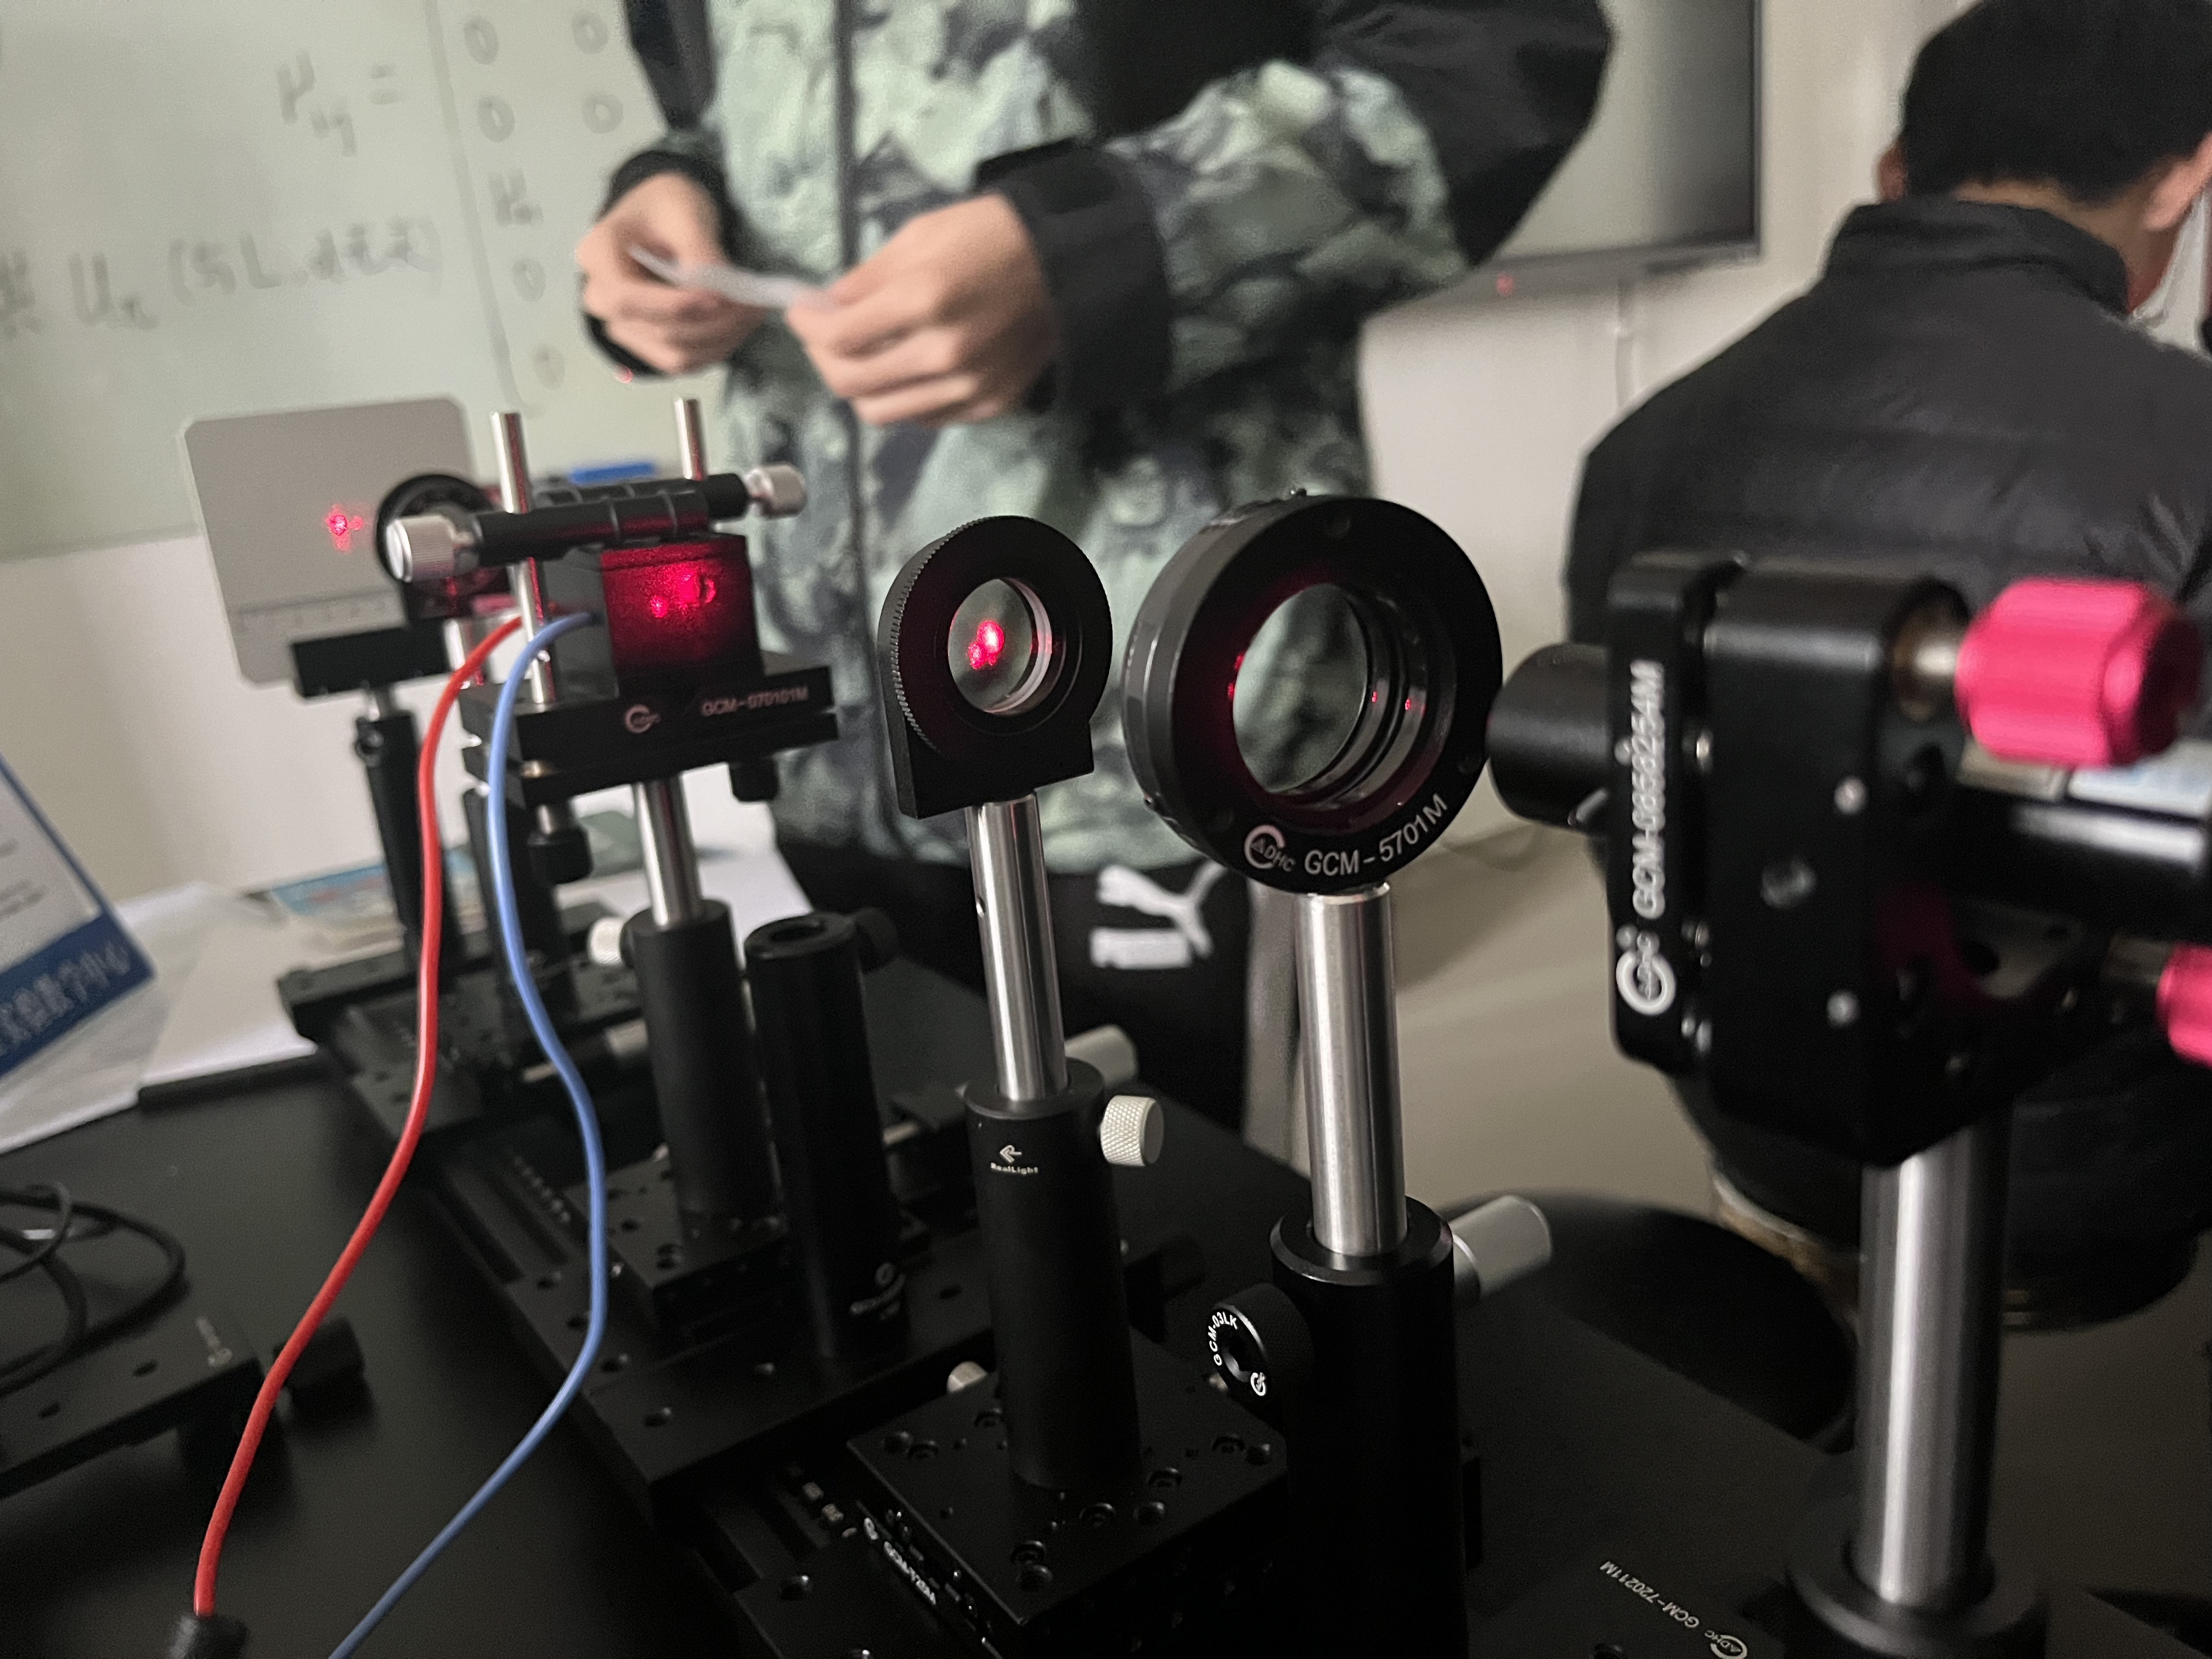
\includegraphics[width=0.5\textwidth]{调节光路.jpg}
		\caption{光路调节示意图}
		\label{fig:optical_path}
	\end{figure}

	放入起偏器和检偏器，调节至正交消光状态。
	然后在光路中放入晶体和聚焦镜，观察到清晰的干涉图样，最终可以在白屏上得到图\ref{fig:interference_pattern}所示的图像。

	\begin{figure}[h!]
		\centering
		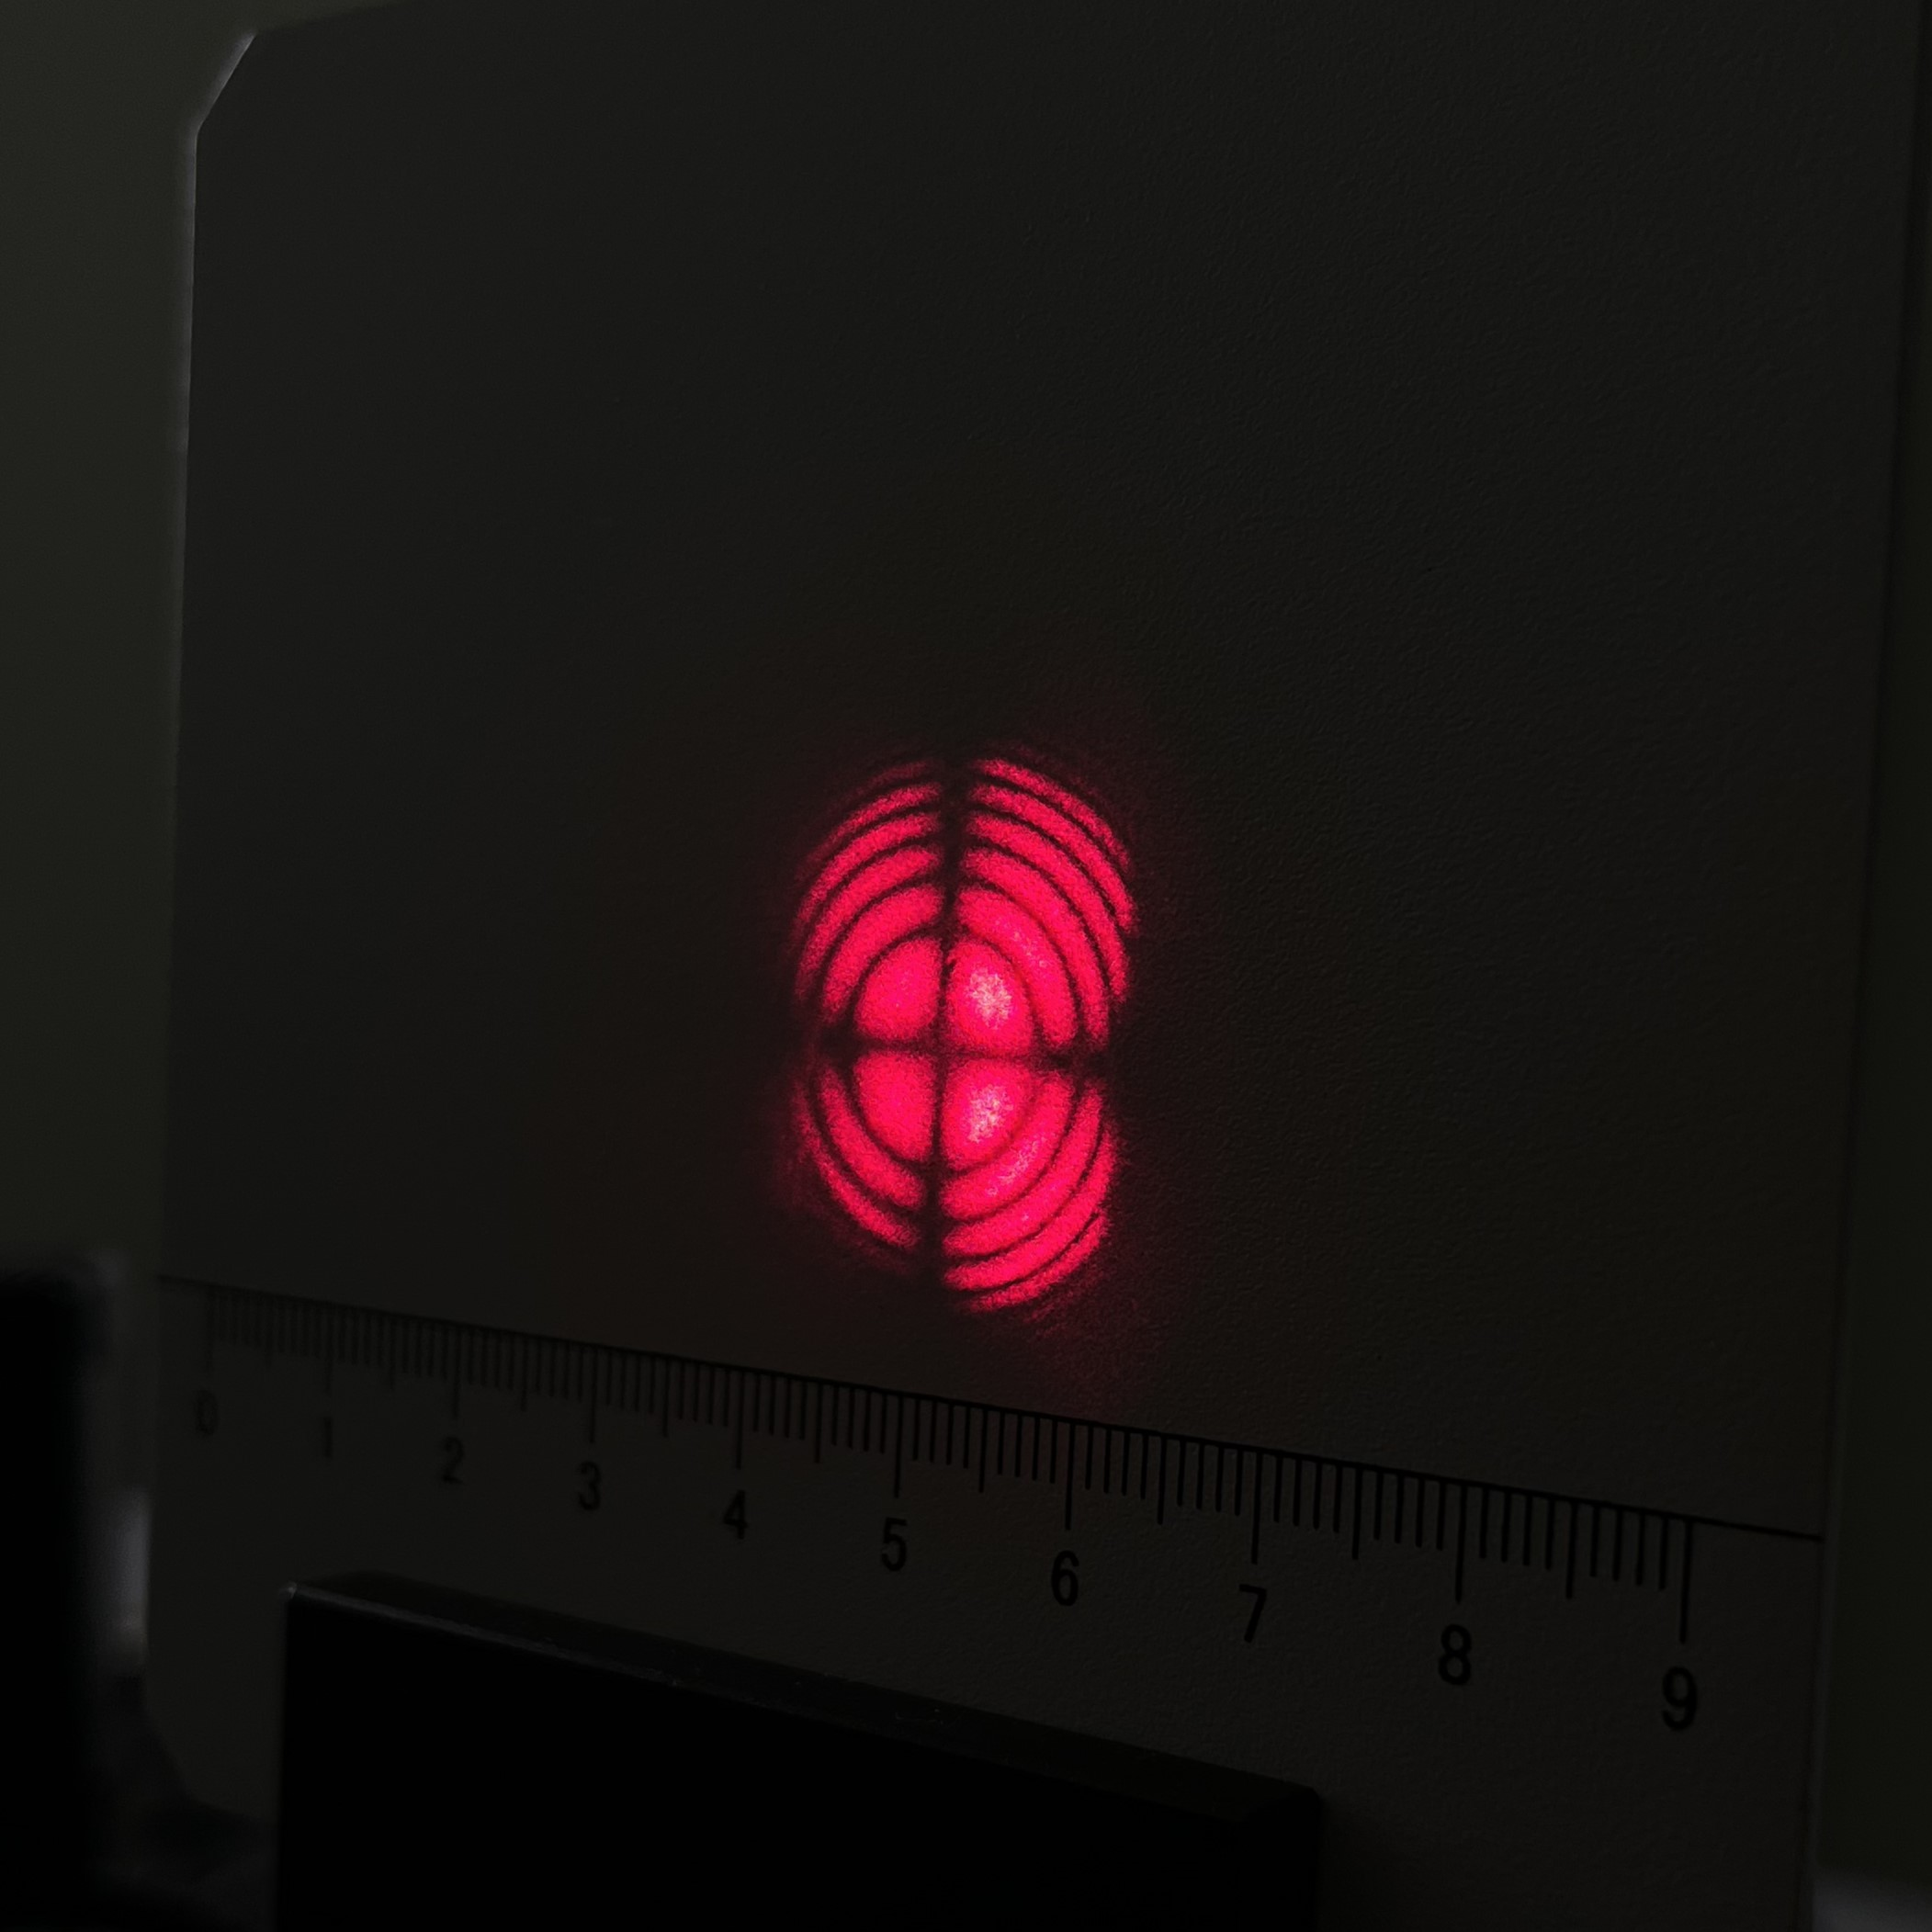
\includegraphics[width=0.5\textwidth]{干涉图样.jpg}
		\caption{铌酸锂晶体干涉图样}
		\label{fig:interference_pattern}
	\end{figure}

	从图中可以得知，我们观察到晶体产生的干涉图样呈现出两条清晰的正交黑色十字线。
	通过微调晶体位置和聚焦镜，使十字线达到最清晰。
	然后缓慢旋转起偏器和检偏器，使黑色十字线分别与水平和竖直方向对齐，确保光路处于最佳工作状态。

	之后我们需要用镜头纸代替凸透镜置于电光晶体前，在检偏器后放置观察白屏，微调晶体的位置使得激光束光斑和黑色十字中心保持重合，如图\ref{fig:alignment}所示。

	\begin{figure}[h!]
		\centering
		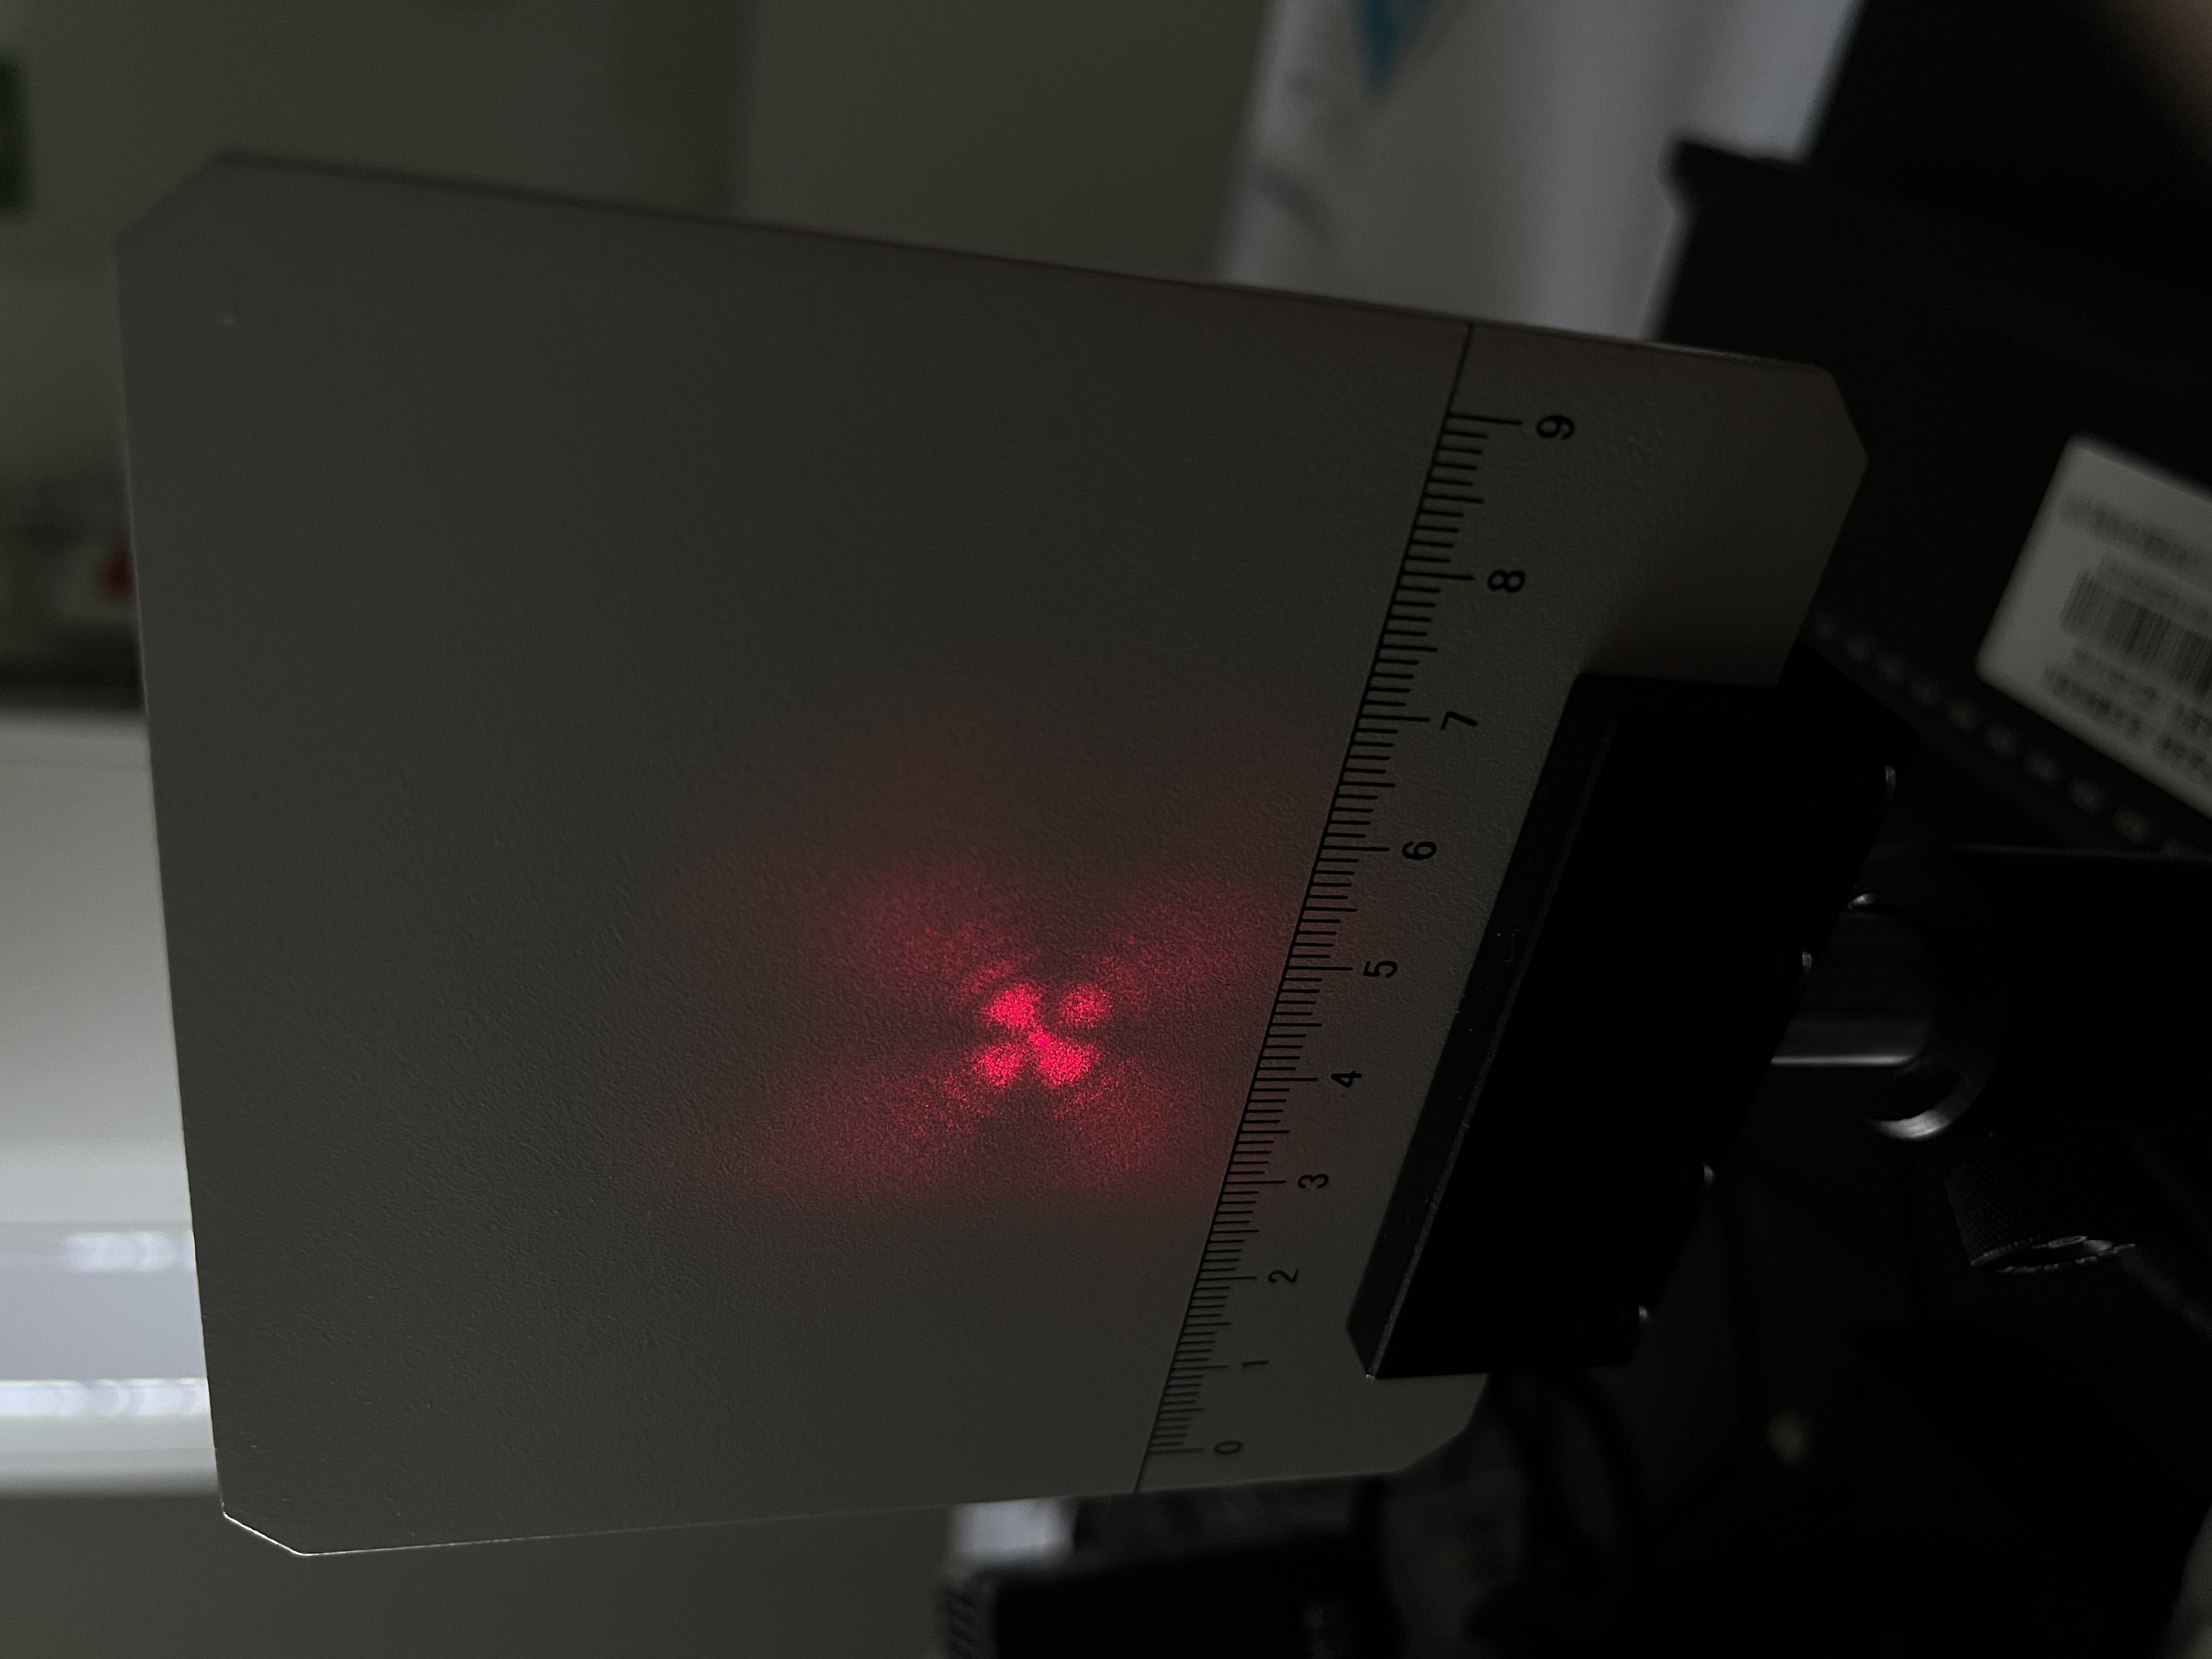
\includegraphics[width=0.5\textwidth]{调节重合.jpg}
		\caption{激光束光斑与黑色十字中心重合调节示意图}
		\label{fig:alignment}
	\end{figure}

	\paragraph{(三)实验测量$V-I$曲线和半波电压}
	经过上述步骤的精细调节，我们已确保激光束与光路系统严格准直，干涉图样清晰稳定，黑色十字中心与光斑完全重合。
	此时光路系统基本处于最佳工作状态，这为后续精确测量半波电压等实验数据奠定了良好基础。
	
	然后使用直流档位测量半波电压，记录输出功率数据。不断调节偏置电压的大小并记录电压值和光强值，测量电光调制的$I-V$曲线（具体测量数据于附录中）。
	值得一提的是，我们在测量时为了减少随机误差带来的影响采用了正向加电压测量和反向减小电压测量并多次测量的方式，有关的原始数据在报告末尾有所体现。

	\begin{figure}[h!]
		\centering
		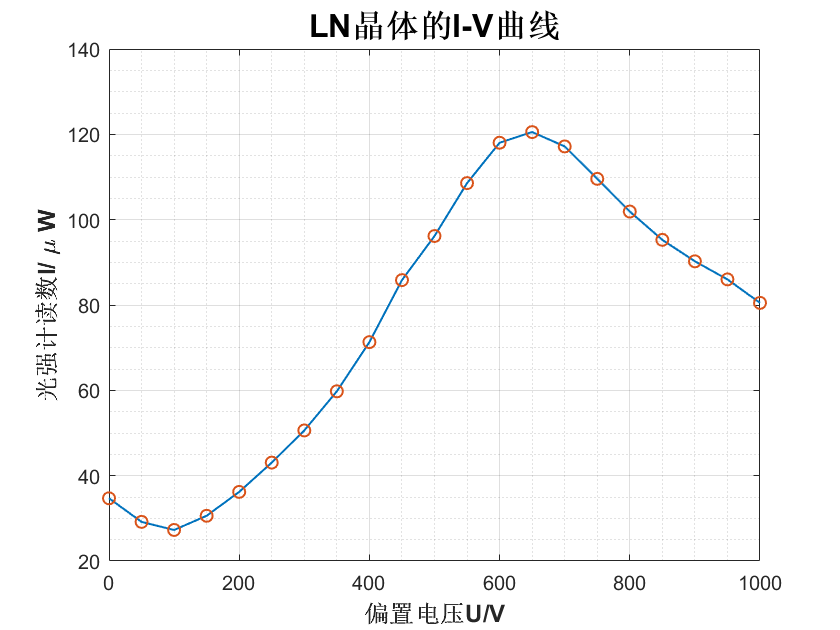
\includegraphics[width=0.5\textwidth]{VI曲线.png}
		\caption{铌酸锂晶体电光调制$I-V$特性曲线}
		\label{fig:IV_curve}
	\end{figure}

	根据图\ref{fig:IV_curve}所示的$I-V$特性曲线，我们可以观察到在测量范围捏，随着外加电压的增大，输出光强呈现正弦式变化。
	这种变化规律与电光调制理论预测的结果一致，验证了铌酸锂晶体的电光效应特性。

	\paragraph{(四)数据处理和半波电压计算}
	随后我们在极值点附近加细测量步长，更加精确地测量晶体的半波电压。
	实验测得半波电压为 $ 620 \mathrm{V} $，与理论值 $ 657.26 \mathrm{V} $ 相比，相对误差为 $ 5.67\% $，表明实验结果与理论预测较为吻合。
	
	我们将数据导出后用正弦函数拟合的方式再次测量了晶体的半波电压，拟合图像如图\ref{fig:sin_fit}所示。
	结合图\ref{fig:sin_fit}所示的拟合曲线，我们可以清晰地看到输出光强随外加电压呈正弦变化，这与电光调制理论一致，进一步验证了铌酸锂晶体的电光效应特性。

	\begin{figure}[h!]
		\centering
		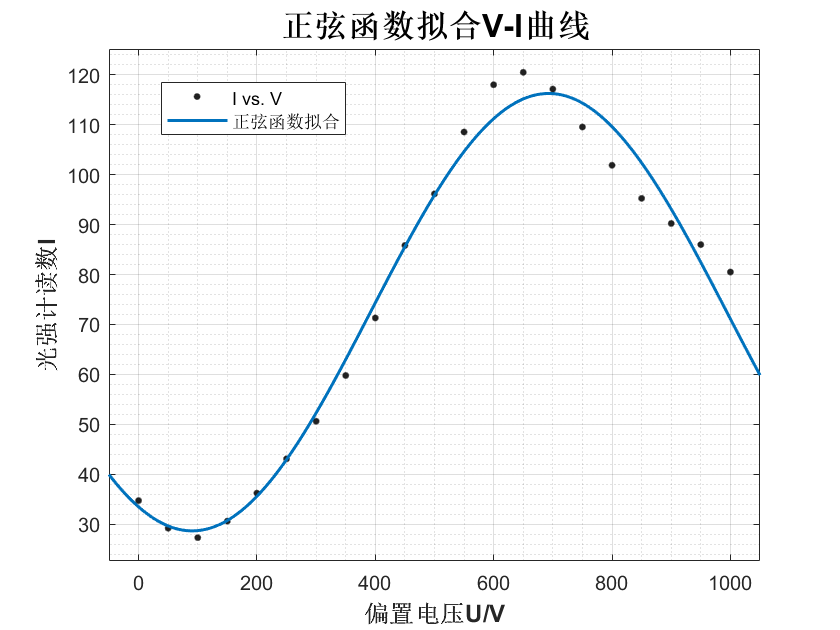
\includegraphics[width=0.5\textwidth]{正弦拟合.png}
		\caption{铌酸锂晶体电光调制正弦拟合曲线}
		\label{fig:sin_fit}
	\end{figure}

	通过拟合的方式我们测得的半波电压为 $ 654 \mathrm{V} $ ，
	这个数值是与理论值 $ 657.26 \mathrm{V} $ 较为接近的，相对误差仅为 $ 0.50\% $。
	相比直接测量得到的 $ 620 \mathrm{V} $，拟合结果显著提高了测量精度。
	这主要是因为正弦函数拟合能够有效消除实验中的随机误差，更好地反映电光调制的规律。
	
	\paragraph{(五)误差分析}
		在本实验中，误差分析主要考虑了实验环境和操作者的影响。
		首先，实验室的光噪音可能会对测量结果产生干扰，尤其是在光强较低的情况下，背景光的波动可能导致输出信号的不稳定。
		此外，操作者在调节偏置电压和晶体位置时的微小差异也可能引入系统误差，影响最终的测量结果。

		为了提高实验的准确性，未来可以考虑以下改进方案：
		\begin{itemize}
			\item 优化实验室的光环境，使用更为精密的光屏蔽措施以减少外部光源的干扰。
			\item 采用自动化设备进行电压调节和位置微调，以减少人为操作带来的误差。
			\item 增加多次测量的次数并进行统计分析，可以更好地评估和降低随机误差的影响，从而提高实验结果的可靠性。
		\end{itemize}

	\subsubsection*{2.加$ \lambda/4 $ 波片之后测量 $ I-V $ 曲线 }
	\paragraph*{(一)实验上确定光轴之间的夹角}
	我们由马吕斯定律不难算出，出射光强满足
	\[ I \propto \sin \theta \cos \theta \]
	因此只要通过光功率计测量保证出射光强达到极大值时，此时即有波片与偏振片夹角为 $45^\circ$，
	倘若不利于光功率计，我们也可以利用两个光强极小值点的中间位置保证以上结果，但并没有光功率计所具有的精确性。

	\paragraph*{(二)测量$ I-V $ 曲线来确定相位变化}
	我们采取之前的测量方法，首先调节偏置电压至零位，然后以固定步长逐步增加电压，同时记录对应的光强值。
	为确保数据可靠性，我们重复测量三次，取平均值作为最终结果。

	\begin{figure}[h!]
		\centering
		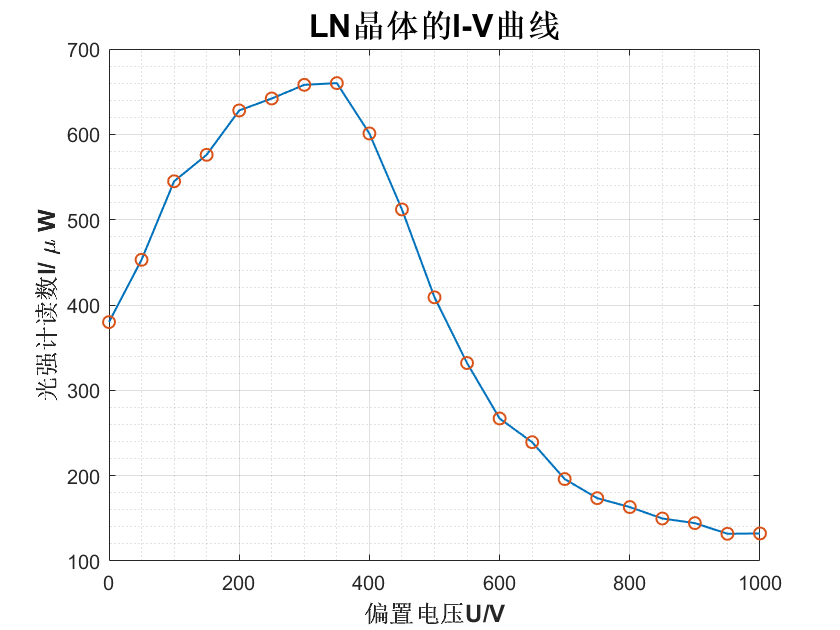
\includegraphics[width=0.5\textwidth]{lambda4.png}
		\caption{加入$\lambda/4$波片后的$I-V$特性曲线}
		\label{fig:lambda4}
	\end{figure}

	经过与上一步相同的数据处理，我们可以得到加入 $ \lambda/4 $ 波片之后的半波电压约为 $ 300 \mathrm{V} $。

	\paragraph*{(三)结果分析与误差讨论}

	通过对比加入$\lambda/4$波片前后的实验结果，我们可以得出以下结论：
	\begin{itemize}
		\item 加入$\lambda/4$波片后，半波电压从$620\mathrm{V}$降低至$300\mathrm{V}$，这与理论预期相符。$\lambda/4$波片的引入改变了光场的偏振态，使得达到相同相位差所需的电压降低。
		\item 实验测得$300\mathrm{V}$的半波电压与理论值存在一定偏差，这主要源于以下因素：
		\begin{enumerate}
			\item $\lambda/4$波片的安装角度可能存在微小偏差，导致其补偿效果不完全理想；
			\item 实验过程中环境温度的变化可能影响晶体的电光系数，从而引入系统误差；
			\item 测量仪器的精度限制，特别是电压源的稳定性和光功率计的分辨率，都会对最终结果产生影响。
		\end{enumerate}
		\item 从图\ref{fig:lambda4}可以看出，$I-V$曲线呈现出良好的线性关系，这表明$\lambda/4$波片的引入有效改善了调制特性，使系统工作在线性调制区。
	\end{itemize}

	为进一步提高实验精度，建议采取以下改进措施：
	\begin{itemize}
		\item 使用更高精度的角度调节装置，确保$\lambda/4$波片的安装角度准确；
		\item 在恒温环境下进行实验，以消除温度变化对晶体特性的影响；
		\item 采用更高精度的测量仪器，如数字示波器配合光电探测器，以提高数据采集的准确性。
	\end{itemize}
	
	\subsubsection*{3.利用光探测器研究调制波形的影响}
	\paragraph*{(一)倍频失真的观察和研究}
	对于倍频失真，其实际上是输出相对于输入波形的频率为两倍时的失真，其一般发生于一个约为二次函数谷底的响应区间，且输入波形为正弦波。
	由于二次函数谷底的非线性，能够使得输入波形零点附近的近似线性变为弧形波形，
	并且在二次函数边缘的线性区又能够保证调制信号的波峰和波谷保持正弦波形式，从而能够输出一个近似为频率翻倍的正弦波。

	具体的理论公式已经在上文中的实验原理部分给出，这里不再赘述。

	在本实验中，按照之前的半波电压测量和有关的分析，我们预计会在 $100\mathrm{V} $ 附近和$630\mathrm{V} $附近出现倍频失真。
	实验测量效果如图\ref{fig:distortion}所示

	\begin{figure}[htbp]
		\centering
		\subfloat[失真1]{\label{fig:distortion1}
		\includegraphics[width=0.45\textwidth]{失真1.png}%调节这里的图片宽度
		}%
		\subfloat[失真2]{\label{fig:distortion2}
		\includegraphics[width=0.45\textwidth]{失真2.png}%调节这里的图片宽度
		}%
		\caption{倍频失真实验测量结果}
		\label{fig:distortion}
	\end{figure}

	其中图\ref{fig:distortion1}对应的偏置电压为$126\mathrm{V} $，图\ref{fig:distortion2}对应的偏置电压为$707\mathrm{V} $。
	这与我们的理论预期比较接近但是有不小的差异，我们认为其主要原因是：
	\begin{enumerate}
		\item 实验分两周完成，两次实验时的温度、湿度等环境条件存在差异，这可能导致晶体电光系数和光学系统性能发生变化；
		\item 实验开展的时间不同，导致环境中的背景光噪声不同，对光强测量结果造成不同程度的影响；
		\item 人为操作因素，两次实验中波片安装角度等光路的细节难以严格控制，这些会引入实验误差；
		\item 实验仪器（如电压源、光功率计等）在不同时间段的性能可能存在微小波动。
	\end{enumerate}
	
	\paragraph*{(二)研究$\lambda/4$波片对调制波形的影响}
	我们分别在两种电压下将$\lambda/4$波片以$45^\circ$为间隔旋转$360^\circ$，观察调制波形的变化。
	
	\begin{figure}[h!]
		\centering
		\includegraphics[width=0.5\textwidth]{旋转.png}
		\caption{$400\mathrm{V}$电压下$\lambda/4$波片旋转$45^\circ$调制波形}
		\label{fig:turnning}
	\end{figure}

	从图\ref{fig:turnning}中可以看出，$\lambda/4$波片的旋转角度对调制波形有显著影响。在实验过程中，我们观察到以下几个主要的误差来源：
	\begin{enumerate}
		\item $\lambda/4$波片的角度调节精度有限，手动旋转可能存在±2°的误差，这直接影响了调制效果的准确性；
		\item 光路系统的稳定性问题，在旋转波片过程中可能引起光路微小偏移，导致测量结果产生波动；
		\item 光电探测器的响应特性存在非线性，特别是在信号较弱时，可能导致波形失真；
		\item 示波器的触发设置和显示参数的选择也会对波形的观测结果产生影响；
		\item 环境光干扰和温度波动可能导致测量基线漂移，影响波形的准确记录。
	\end{enumerate}

	\paragraph*{(三)光通讯模拟实验}
	最后我们进行光通讯模拟实验，利用MP3连接控制器的外调端口，并将光探测器与音响连接。
	通过MP3播放音乐，可以观察到音响发出声音与音乐的基本一致，适当调节偏置电压，我们可以音响中听到非常清晰的音乐，说明晶体处于线性工作区。
	
	同样当我们将偏置电压调节到失真的区域时，我们无法听到清晰的音乐，说明晶体处于非线性工作区，如图\ref{fig:distortion3}所示。	
	\begin{figure}[h!]
		\centering
		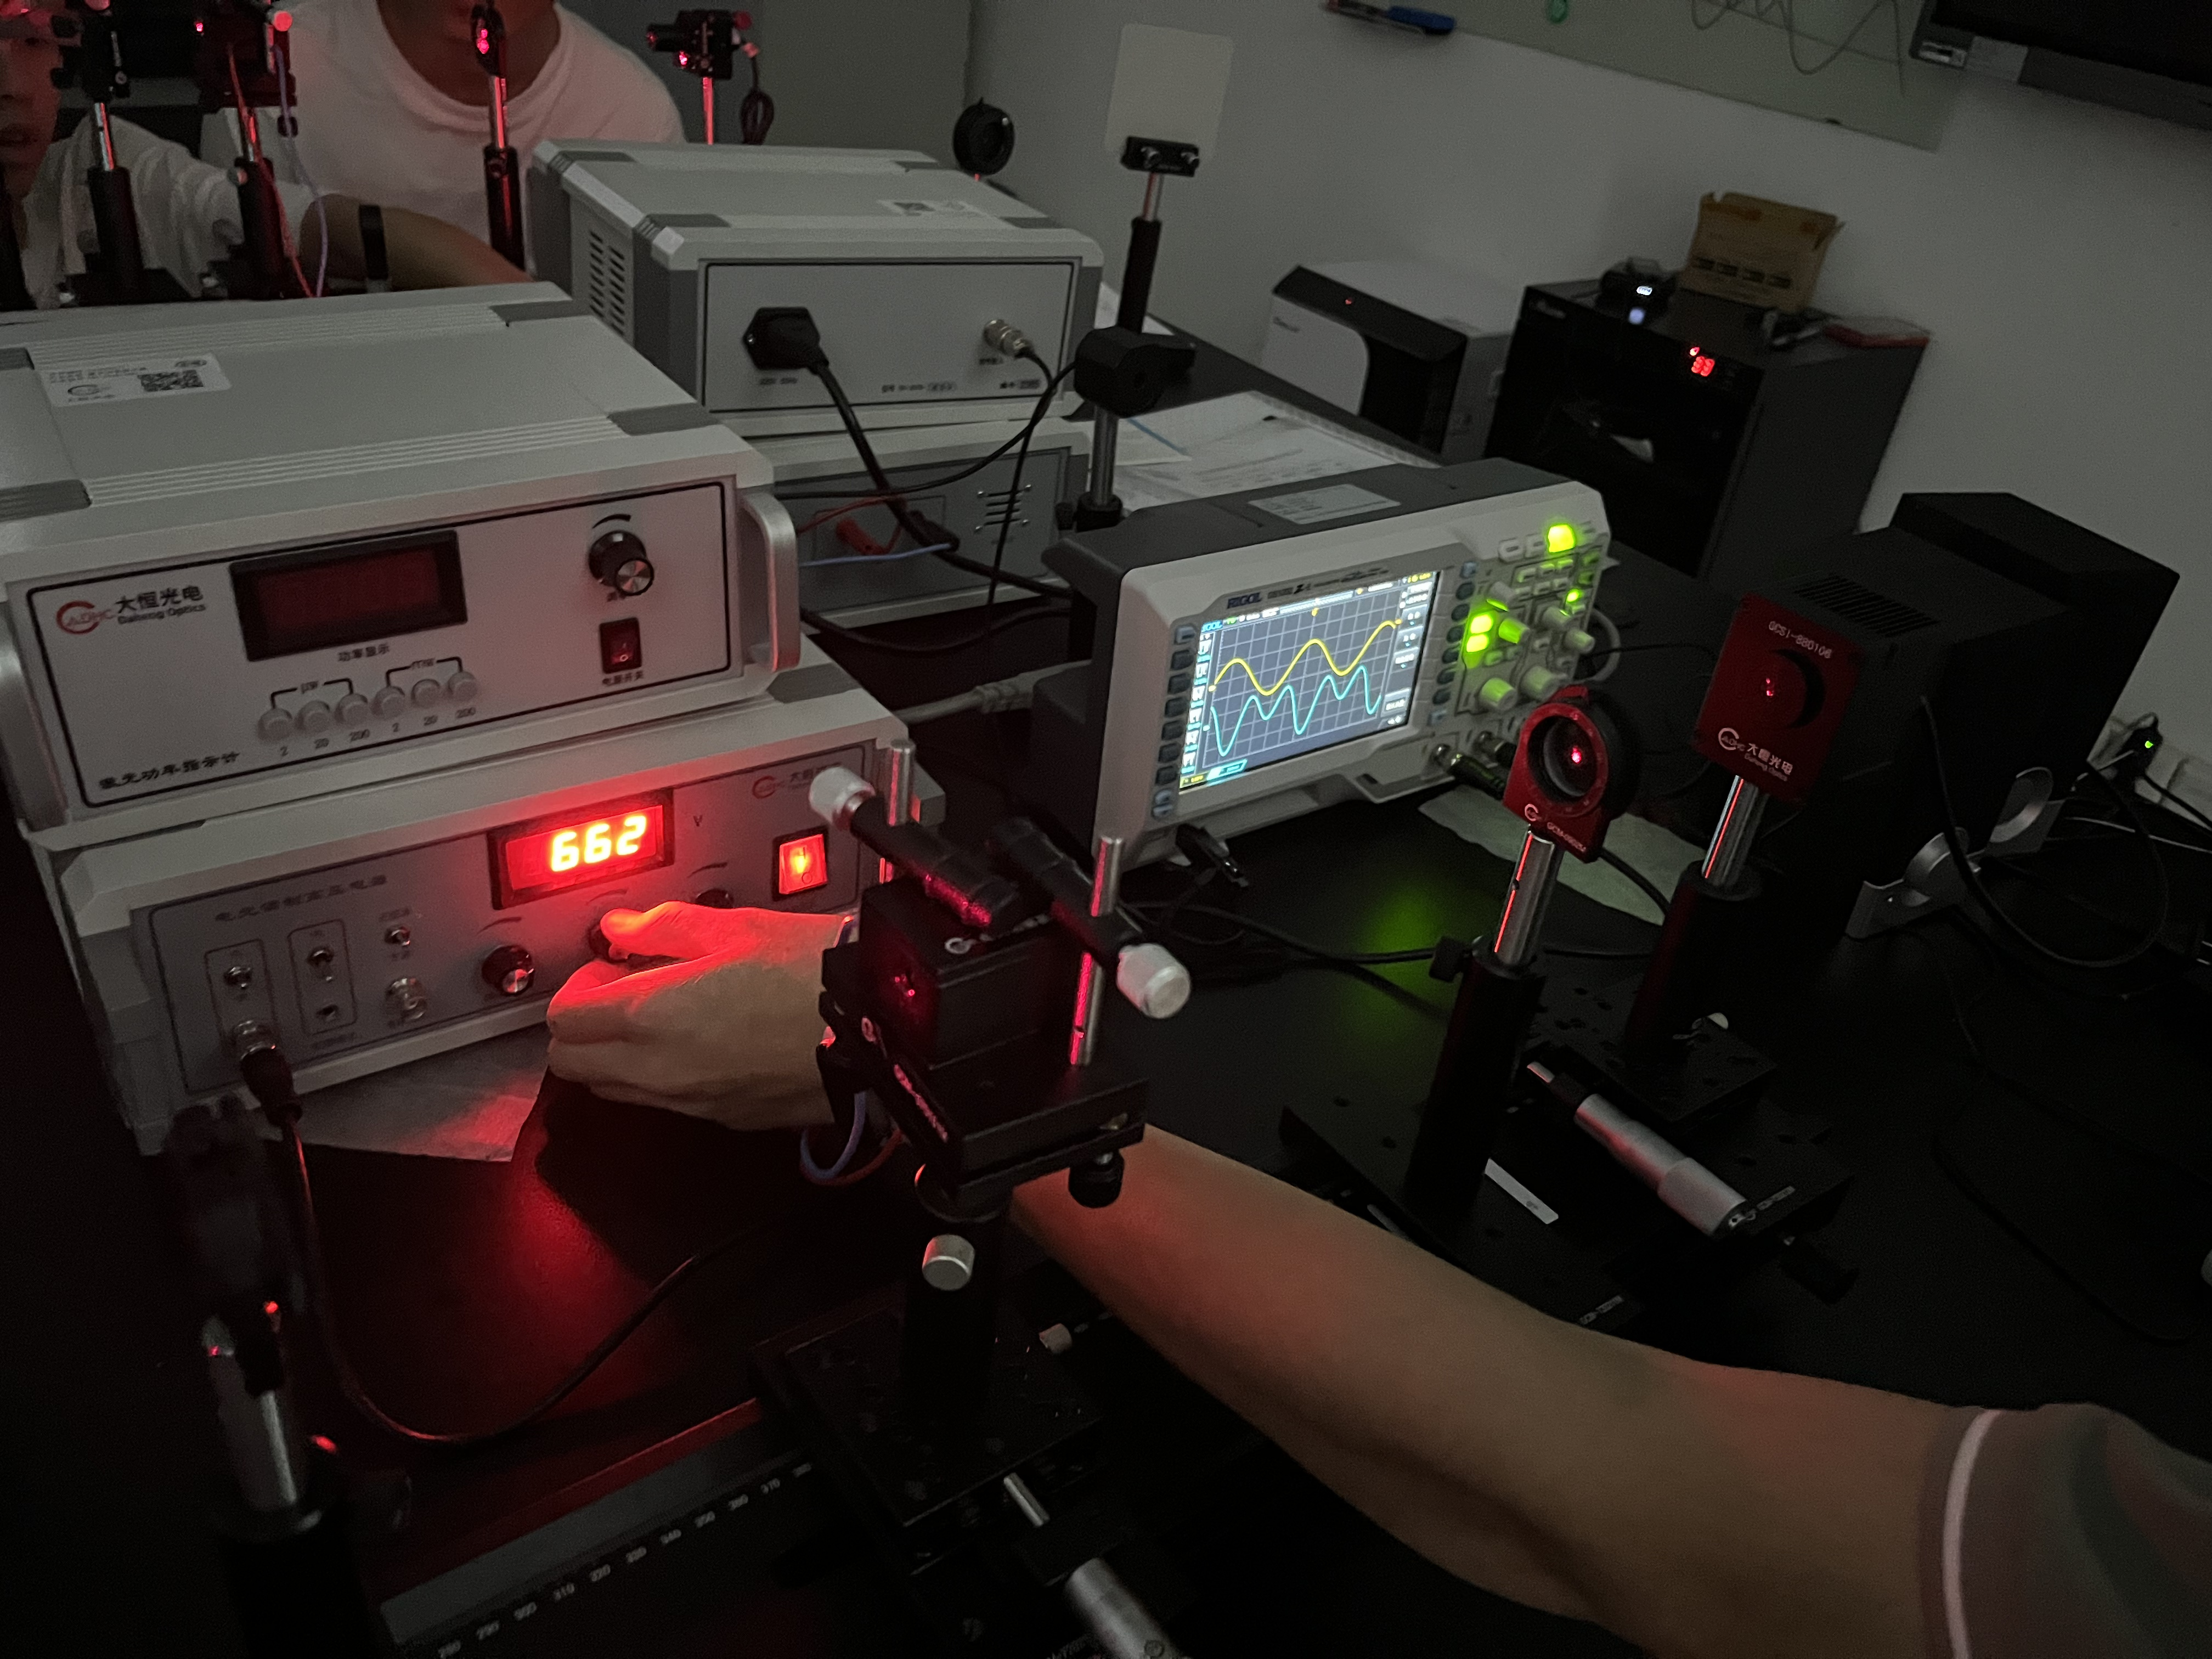
\includegraphics[width=0.5\textwidth]{失真3.jpg}
		\caption{非线性工作区的调制波形}
		\label{fig:distortion3}
	\end{figure}

	在加入1/4波片后，同样可以发现，在线性区位置音箱能够输出清晰的声音，旋转波片声音会呈现“清晰-不清晰-清晰”的周期性变化。
	
\subsection*{【思考题】}
\subsubsection*{计算磷酸二氘钾（KD*P）晶体的半波电压，并证明其与晶体尺寸无关}

对于磷酸二氘钾（KD*P）晶体，其电光系数矩阵为：
\[
\gamma_{ij} =
\begin{bmatrix}
0 & 0 & 0 \\
0 & 0 & 0 \\
0 & 0 & 0 \\
\gamma_{41} & 0 & 0 \\
0 & \gamma_{52} & 0 \\
0 & 0 & \gamma_{63}
\end{bmatrix}
\]

在纵向电光效应（外加电场方向与光传播方向一致）情况下，电光效应引起的相位延迟为：
\[
\delta = \frac{2\pi}{\lambda} L \Delta n
\]
其中，折射率变化量：
\[
\Delta n = \frac{1}{2} n_0^3 \gamma_{63} E_z
\]
外加电场 $E_z$ 可表示为：
\[
E_z = \frac{U}{L}
\]
因此，相位延迟 $\delta$ 可写为：
\[
\delta = \frac{2\pi}{\lambda} L \cdot \frac{1}{2} n_0^3 \gamma_{63} \frac{U}{L}
\]
当 $\delta = \pi$ 时，对应的半波电压 $U_\pi$ 为：
\[
U_\pi = \frac{\lambda}{n_0^3 \gamma_{63}}
\]
从该表达式可以看出，半波电压 $U_\pi$ **仅与晶体的材料参数（$n_0$ 和 $\gamma_{63}$）及光的波长 $\lambda$ 相关，而与晶体的尺寸（长度 $L$ 和厚度 $d$）无关**。

\subsubsection*{电光晶体的光轴与激光束不平行，或者电光晶体的 $x$ 轴、$y$ 轴分别与起偏器、检偏器不平行的影响}

\paragraph*{(一)如何检查}
\begin{enumerate}
    \item \textbf{观察干涉图样}：
    若光轴与激光束不平行，则透过光的干涉条纹可能发生倾斜或畸变，黑色十字形干涉图样可能偏离中心或不对称。
    \item \textbf{旋转晶体观察变化}：
    轻微旋转电光晶体，若观察到干涉条纹明显变化，则表明光轴未严格平行于激光束。
    \item \textbf{调整起偏器和检偏器方向}：
    逐步调整起偏器与检偏器的偏振方向，使消光最优，并观察干涉条纹的变化。如果黑色十字始终不规则，说明晶体的主轴方向可能未正确对准。
\end{enumerate}

\paragraph*{(二)对测量结果的影响}
\begin{enumerate}
    \item \textbf{光轴与激光束不平行的影响}：
    由于入射光的传播方向与晶体光轴不一致，导致双折射效应与理论计算存在偏差，从而影响相位差计算，使得测得的半波电压 $U_\pi$ 误差增大。
    \item \textbf{起偏器、检偏器未与晶体轴对齐的影响}：
    若起偏器或检偏器的方向未正确对齐晶体的 $x$ 轴、$y$ 轴，则通过晶体的光分量不符合理论预测，影响消光比测量，从而影响电光调制器的透过率测量和线性工作区确定。
\end{enumerate}

\subsection*{【原始数据的记录】}
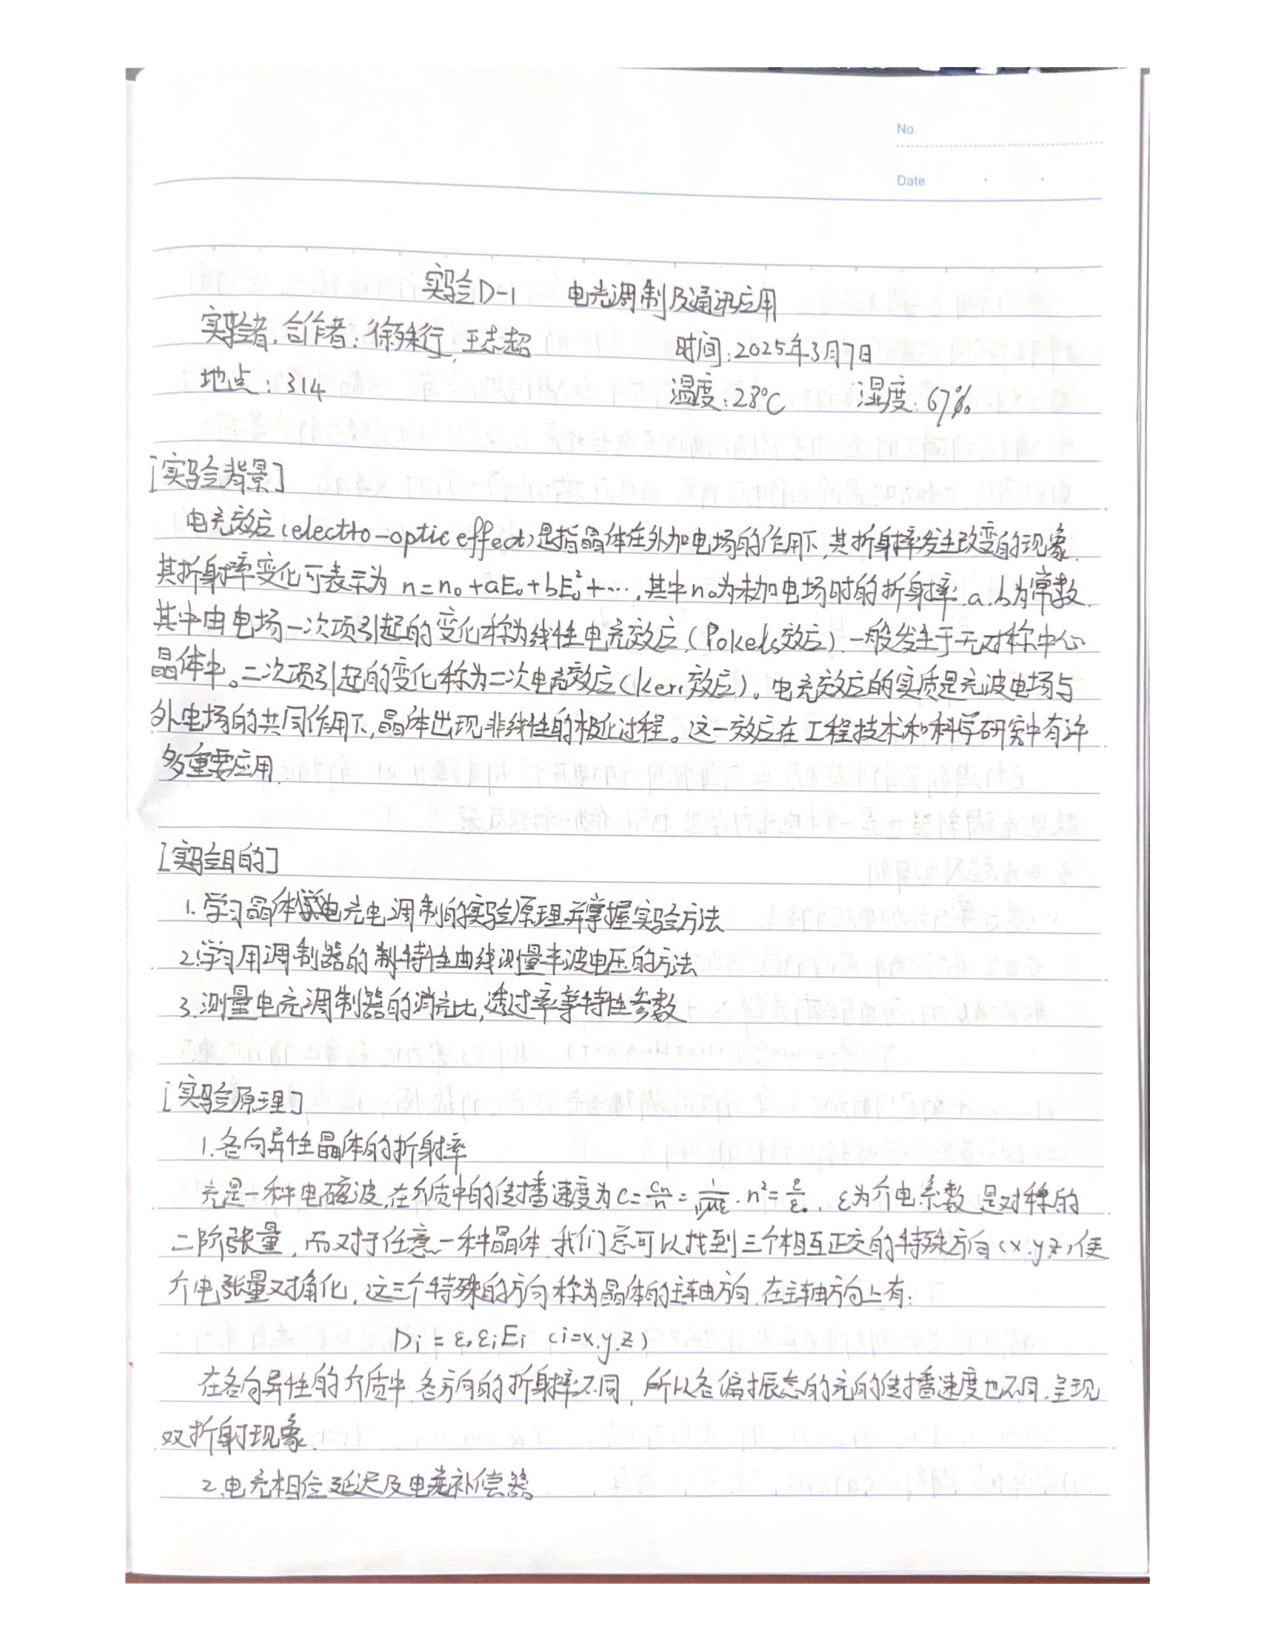
\includepdf[pages=-]{电光调制scan.pdf}

\end{document}
